\documentclass[a4paper,10pt]{article}
\usepackage[utf8]{inputenc}
\usepackage{tikz}
\usepackage{amsmath}
\usepackage{fullpage}

%opening
\title{Attaque du protocole de l'équipe AKJ-SEP}
\author{par l'Equipe Stone Jaws}
\date{9 octobre 2018}

\begin{document}

\maketitle

\section{Le protocole}

Considérons 3 rôles $i$, $r$, et $m$ (que l'on appellera respectivement initiateur, récepteur, et serveur). La sémantique (en utilisant les notations de \cite{cas}) de ce protocole est alors donnée par :
\begin{eqnarray*}
	TdSD(i) & = & \{ (i,r,m, K, K_{im}), \\
		& & \texttt{send}_1(i,m, \textrm{senc}(\langle r, K \rangle,K_{im}) ),\\
		& & \texttt{recv}_4(m,i, \textrm{senc}(h(K), K_{im}))\}
\end{eqnarray*}
\begin{eqnarray*}
	TdSD(r) & = & \{ (i,r,m, K_{rm}), \\
		& & \texttt{recv}_2(m,r, \textrm{senc}(\langle i, K \rangle,K_{rm}) ),\\
		& & \texttt{send}_3(r,m, \textrm{senc}(\langle i, h(K) \rangle,K_{rm}) )\}
\end{eqnarray*}
\begin{eqnarray*}
	TdSD(m) & = & \{ (i,r,m, K_{rm}, K_{im}), \\
		& & \texttt{recv}_1(i,m, \textrm{senc}(\langle r, K \rangle,K_{im}) ),\\
		& & \texttt{send}_2(m,r, \textrm{senc}(\langle i, K \rangle,K_{rm}) ),\\
		& & \texttt{recv}_3(r,m, \textrm{senc}(\langle i, h(K) \rangle,K_{rm}) ),\\
		& & \texttt{send}_4(m,i, \textrm{senc}(h(K), K_{im}))\}
\end{eqnarray*}


\begin{center}

\begin{figure}
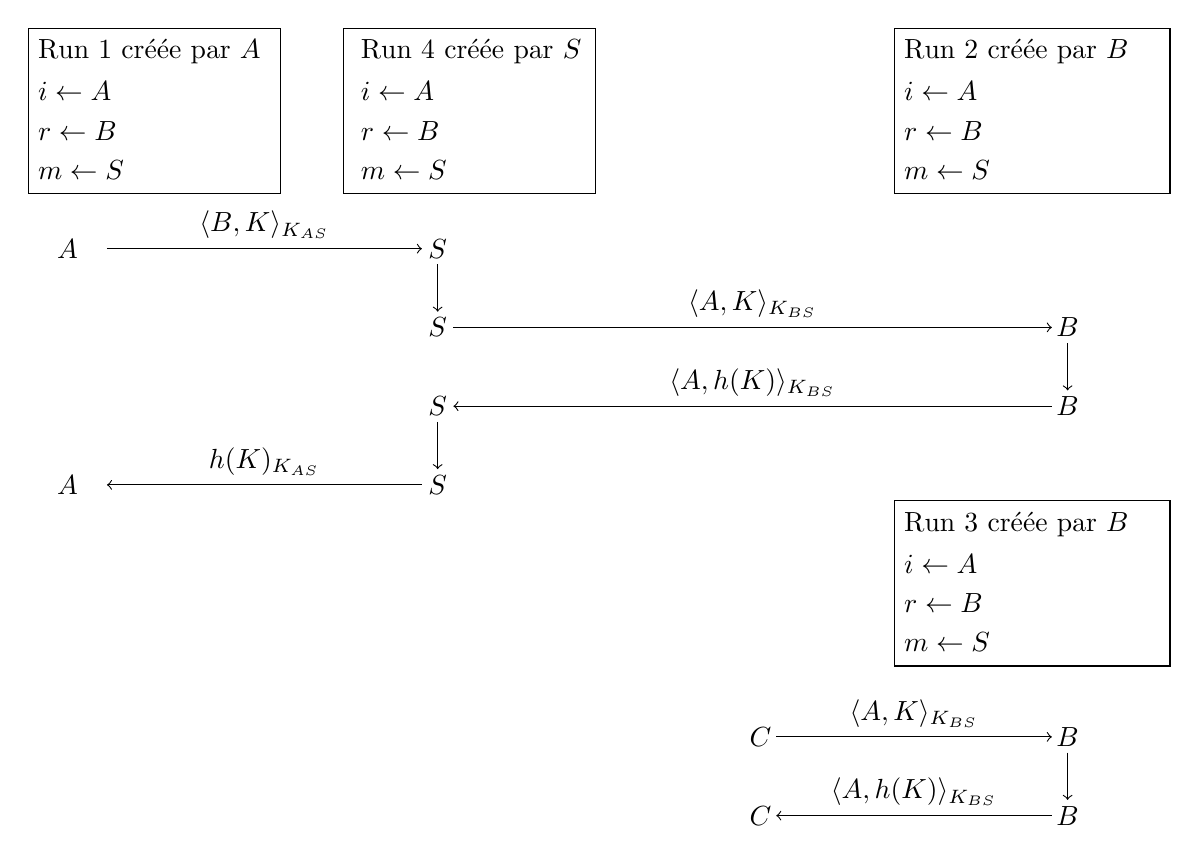
\begin{tikzpicture}
  \draw(-7,8.8) rectangle (-3.8,6.7);
	\draw (-7,8.5) node[right]{Run 1 créée par $A$};
	\draw (-7,8) node[right]{$i \leftarrow A$};
	\draw (-7,7.5) node[right]{$r \leftarrow B$};
	\draw (-7,7) node[right]{$m \leftarrow S$};

  \draw(-3,8.8) rectangle (0.2,6.7);
	\draw (-2.9,8.5) node[right]{Run 4 créée par $S$};
	\draw (-2.9,8) node[right]{$i \leftarrow A$};
	\draw (-2.9,7.5) node[right]{$r \leftarrow B$};
	\draw (-2.9,7) node[right]{$m \leftarrow S$};

	\draw(4,8.8) rectangle (7.5,6.7);
	\draw (4,8.5) node[right]{Run 2 créée par $B$};
	\draw (4,8) node[right]{$i \leftarrow A$};
	\draw (4,7.5) node[right]{$r \leftarrow B$};
	\draw (4,7) node[right]{$m \leftarrow S$};

	\draw (-6.5,6) node{$A$} ;
	\draw[->]  (-6,6) -- node[above]{$\langle B, K\rangle_{K_{AS}}$} (-2,6) ;
	\draw (-1.8,6) node{$S$} ;
	\draw[->]  (-1.8,5.8) -- (-1.8,5.2) ;
	\draw (-1.8,5) node{$S$} ;
	\draw[->]  (-1.6,5) -- node[above]{$\langle A, K\rangle_{K_{BS}}$} (6,5) ;
	\draw (6.2,5) node{$B$} ;
	\draw[->]  (6.2,4.8) -- (6.2,4.2) ;
	\draw (6.2,4) node{$B$} ;
	\draw[<-]  (-1.6,4) -- node[above]{$\langle A, h(K)\rangle_{K_{BS}}$} (6,4) ;
	\draw (-1.8,4) node{$S$} ;
	\draw[->]  (-1.8,3.8) -- (-1.8,3.2) ;
	\draw (-1.8,3) node{$S$} ;
	\draw[<-]  (-6,3) -- node[above]{$h(K)_{K_{AS}}$} (-2,3) ;
	\draw (-6.5,3) node{$A$} ;

	\draw(4,2.8) rectangle (7.5,0.7);
	\draw (4,2.5) node[right]{Run 3 créée par $B$};
	\draw (4,2) node[right]{$i \leftarrow A$};
	\draw (4,1.5) node[right]{$r \leftarrow B$};
	\draw (4,1) node[right]{$m \leftarrow S$};

	\draw (2.3,-0.2) node{$C$} ;
	\draw[->]  (2.5,-0.2) -- node[above]{$\langle A, K\rangle_{K_{BS}}$} (6,-0.2) ;
	\draw (6.2,-0.2) node{$B$} ;
	\draw[->]  (6.2,-0.4) -- (6.2,-1) ;
	\draw (6.2,-1.2) node{$B$} ;
	\draw[<-]  (2.5,-1.2) -- node[above]{$\langle A, h(K)\rangle_{K_{BS}}$} (6,-1.2) ;
	\draw (2.3,-1.2) node{$C$} ;
\end{tikzpicture}
\caption{Attaque du protocole AKJ-SEP}
\label{fig1}
\end{figure}
\end{center}

\section{Attaque sur le protocole}
L'attaque ne commence après une première execution du protocole entre les agents $A$ (avec une run $1$) et $B$ (avec une run $2$). Cet échange se passe sans encombre, mais tous les messages ont été vus par l'attaquant $C$.
Celui-ci va alors tromper l'agent $B$ avec les étapes suivantes. $B$ commence une run $3$ avec $A$ comme initiateur et $B$ comme recepteur.
\begin{enumerate}
\item $C$ envoie le message $\langle A, K \rangle_{K_{BS}}$ à $B$ en se faisant passer pour $S$.
\item $B$ répond par $\langle A, h(K) \rangle_{K_{BS}}$ à destination de $S$. Mais ce message est bloqué par l'attaquant.
\end{enumerate}
À la fin, $B$ pense donc avoir communiqué avec $A$ une deuxième fois, alors que $A$ n'est jamais intervenu.

On remarque alors qu'une des propriétés exigées n'est pas vérifiée :
le récepteur $B$ de la run $3$ croit recevoir une donnée d'un initiateur $A$ qui ne l'a en fait jamais envoyée.
\end{itemize}

\bibliographystyle{plain}
\bibliography{ref.bib}

\end{document}
